\documentclass{article}
\usepackage{graphicx}
\usepackage{hyperref}
\usepackage[a4paper, margin=1.25in]{geometry}
\usepackage{breakcites}
\usepackage{subcaption}
\usepackage{float}
\usepackage{textcomp}
\usepackage{amsmath}
\usepackage{textgreek}
\usepackage{authblk}
\usepackage{rotating}
\usepackage{booktabs}
\usepackage{longtable}

\begin{document}

\title{Modeling the Food Insecurity Experience Scale (FIES) in the Present and Future}

\author[1]{Matthew Cooper}
\author[2]{Benjamin Müller}

\affil[1]{T.H. Chan School of Public Health, Harvard University}
\affil[2]{Department of Economics, Vienna University of Economics and Business}

\maketitle
\begin{abstract}
The Food Insecurity Experience Scale (FIES) measures the experiential aspects of food insecurity, and has been selected as a target for the second Sustainable Development Goal (SDG) of Zero Hunger.  Here, we present the preliminary results of our work modeling this indicator globally for the years 2020-2030.

\end{abstract}

\section{Introduction}

\subsection{Measuring Food Security and the Genesis of the FIES}
Food security is a key part of human development, but has traditionally been difficult to measure.  Metrics of macro-health, such as anthropometry and mortality rates are correlated broadly with food insecurity \cite{Puffer1973, Habicht1974}, but are confounded with other determinants of health such as infectious disease.  Other proxies for food security, such as food availability estimated from crop yields \cite{Maxwell1992}, are inadequate because they do not indicate how accessible food is to the general population, and food insecurity can certainly occur in the absence of food availability decline \cite{Sen1983}.

As researchers began to focus on food insecurity at the individual and household level, household microdata collecting information on household finances and consumption became a common proxy for food security \cite{Haddad1994}.  However, these efforts were criticized for being onerous, insufficiently comparable, as well as for ignoring subjective and experiential aspects of food security \cite{Maxwell1996}.  This led to the emergence of several indicators designed to be rapidly deployable, culturally cross-comparable, and based on the lived experience of food security.  These metrics include the Household Food Insecurity and Access Scale (HFIAS) \cite{Coates2007}; the Coping Strategies Index (CSI) \cite{Maxwell1999}; the Household Hunger Scale (HHS) \cite{Ballard2011}; the Food Consumption Score (FCS); and the Household Dietary Diversity Scale (HDDS) \cite{Kennedy2010}.

Drawing on the insights derived in designing and implementing these food security metrics, the Food Insecurity Experience Scale (FIES) was developed by the Food and Agricultural Organization (FAO) of the UN.

\subsection{The FIES}
The FIES asks participants eight questions about their experience of food insecurity during the previous year \cite{Cafiero2018}, collected in countries around the world both in person and over the telephone with the assistance of Gallup World Poll.  These questions are:

\begin{enumerate}
	\item During the last 12 MONTHS, was there a time when you were worried you would not have enough food to eat because of a lack of money or other resources?
	\item Still thinking about the last 12 MONTHS, was there a time when you were unable to eat healthy and nutritious food because of a lack of money or other resources?
	\item Was there a time when you ate only a few kinds of foods because of a lack of money or other resources?
	\item Was there a time when you had to skip a meal because there was not enough money or other resources to get food?
	\item Still thinking about the last 12 MONTHS, was there a time when you ate less than you thought you should because of a lack of money or other resources?
	\item Was there a time when your household ran out of food because of a lack of money or other resources?
	\item Was there a time when you were hungry but did not eat because there was not enough money or other resources for food?
	\item During the last 12 MONTHS, was there a time when you went without eating for a whole day because of a lack of money or other resources?
\end{enumerate}

Based on the responses to these questions, a Rasch model is used to generate the score for the population \cite{Engelhard2013}.  

\section{Data}
For our analysis, we draw on several datasets.  First, we use the individual responses from 335,139 individuals from 331 surveys across 77 countries, downloaded from the FAO microdata catalogue.  Additionally, we use country-level FIES scores downloaded from FAOSTAT.

To disaggregate the FIES by urban-rural areas, we used data on urbanization from \cite{Jiang2017}.

\subsection{Covariates Available in the Present}
We use a large stack of covariates available for the present or the near-present, reflective of factors related to many aspects of food systems.  Datasets that were originally gridded were aggregated to the Admin-1 level taking the mean value.  A full table of datasets is given in Table \ref{tab:covars1}.

\begin{table}[H]
	\begin{tabular}{llll}
		\toprule
		Name & Availability & Scale & Source \\
		\midrule
		Agriculture As A Percentage Of GDP & Annual & National & \cite{TheWorldBank2016} \\
		Net Oda Per Capita & Annual & National & \cite{TheWorldBank2016} \\
		Percent of Area Bare Ground & Annual & Admin-1 & \cite{Song2018} \\
		Percent Of Area With Built Up Land Cover & 2000 \& 2014 & Admin-1 & \cite{Pesaresi2015} \\
		Staple Crop Proction Per Capita & Annual & National & \cite{FAOSTAT2018} \\
		Elevation & Static & Admin-1 & \cite{USGS1996} \\
		Net School Enrollment & Annual & National & \cite{TheWorldBank2016} \\
		Forest Cover & Annual & Admin-1 & \cite{Song2018} \\
		Government Effectiveness Indicator & Annual & National & \cite{Kaufmann2011} \\
		GDP PPP Per Capita & Annual & Admin-1 & \cite{Kummu2018} \\
		HDI & Annual & Admin-1 & \cite{Kummu2018} \\
		Value Of All Imports Per Capita & Annual & National & \cite{TheWorldBank2016} \\
		Irrigated Area & 2000 & Admin-1 & \cite{SiebertS.DollP.FeickS.FrenkenK.Hoogeveen2013} \\
		Time To Travel To A City  & 2015 & Admin-1 & \cite{Uchida2008} \\
		Mean Annual Precipitation & Static & Admin-1 & \cite{Funk2015} \\
		NDVIi & Annual & Admin-1 & \cite{Song2018} \\
		People Per Pixel & 2010, 2015, 2020 & Admin-1 & \cite{Doxsey-Whitfield2015} \\
		Topographic Roughness Index & Static & Admin-1 & \cite{USGS1996, Riley1999} \\
		Political Stability Index & Annual & Admin-1 & \cite{Kaufmann2011} \\
		Number Of Conflict Deaths Within 50Km & Annual & Admin-1 & \cite{Eriksson2015} \\
		Nutritional Diversity Of Agriculture & 2015 & Admin-1 & \cite{Herrero2017a} \\
		Average Maximum Temperature & Roughly Static & Admin-1 & \cite{Sheffield2006} \\
		Number Of Buffaloes Per Square Km & 2010 & Admin-1 & \cite{Robinson2014} \\
		Number Of Cattle Per Square Km & 2010 & Admin-1 & \cite{Robinson2014} \\
		Number Of Chickens Per Square Km & 2010 & Admin-1 & \cite{Robinson2014} \\
		Number Of Ducks Per Square Km & 2010 & Admin-1 & \cite{Robinson2014} \\
		Number Of Horses Per Square Km & 2010 & Admin-1 & \cite{Robinson2014} \\
		Number Of Pigs Per Square Km & 2010 & Admin-1 & \cite{Robinson2014} \\
		Number Of Sheep Per Square Km & 2010 & Admin-1 & \cite{Robinson2014} \\
		Incidence \textit{P. falciparum} Malaria & Annual & Admin-1 & \cite{Weiss2019} \\
		Incidence \textit{P. vivax} Malaria & Annual & Admin-1 & \cite{Weiss2019} \\
		\bottomrule
	\end{tabular}
	\caption{Co-Variates Included in Present-Day Analysis}
	\label{tab:covars1}
\end{table}


\begin{table}[H]
	\begin{tabular}{llll}
		\toprule
		Name & Availability & Scale & Source \\
		\midrule
        HDI & Annual & Subnational & GDL \\
        Life Expectancy & Annual & Subnational & GDL \\
        GNI Per Capita & Annual & Subnational & GDL \\
        Expected Years School & Annual & Subnational & GDL \\
        Mean Years School & Annual & Subnational & GDL \\
        Country Programmable Assistance (CPA) & Annual & National & OECD Database \\
        AG PCT GD & Annual & National & World Bank \\
        Import Value Per Capita & Annual & National & World Bank \\
        Undernourishment & Annual & National & World Bank, FAO \\
        government_effectiveness & Annual & National & World Bank WGIs \\
        control_corruption & Annual & National & World Bank WGIs \\
        regulatory_quality & Annual & National & World Bank WGIs \\
        rule_of_law & Annual & National & World Bank WGIs \\
        stability_noviolence & Annual & National & World Bank WGIs \\
        voice_accountability & Annual & National & World Bank WGIs \\
        mean annual precip & static & subnational & WorldClim \\
        mean average temp & static & subnational & WorldClim \\
        forest cover & 2016 & subnational & Song et al \\
        elevation & static & subnational & ETOPO5 \\
        ruggedness & static & subnational & ETOPO5 \\
        
        %TODO:
        %Nutritional Diversity
        %Malaria
        %Stunting
        %Livestock
        %Buitup
        %Irrigation
        %TTC
        %Sum of conflict deaths
        %Urban-Rural pop
        
        
		\bottomrule
	\end{tabular}
	\caption{Co-Variates Included in Present-Day Analysis NEW}
	\label{tab:covars2}
\end{table}


\subsection{Covariates Available in the Present and Future}
To model the FIES in the future, we use projections from multiple sources. Most covariates are derived in line with the Shared Socio-Economic Pathways (SSPs). The SSPs are a framework to estimate what the future might look like in terms of human development and climate-change mitigation, based on a number of scenarios.  We use projections for SSP2, the middle-of the road pathway, from \cite{Crespo2017}, \cite{Dellink2017}, \cite{Rao2019a}, \cite{KC2017}, \cite{Jiang2017} and \cite{SSPData2017}.
Additionally, we use projections for poverty and water scarcity from \cite{WDL2020PC} and \cite{WDL2020WSC} respectively and estimate our own forecasts (with elasticities to GDP) for ``Imports per capita'' and ``Agriculture as a Percent of GDP'' (See Table \ref{tab:covars3}.


\begin{table}[H]
	\begin{tabular}{llll}
		\toprule
		Name & Availability & Scale & Source \\
		\midrule
		GDP PPP per capita & Annual & National & \cite{Crespo2017} \\
		- & - & - & \cite{Dellink2017} \\
		Gini index & Annual & National & \cite{Rao2019a} \\
		Share primary education & Annual & National & \cite{KC2017} \\
		Share secondary education & Annual & National & \cite{KC2017} \\
		%Share tertiary education & Annual & National & \cite{KC2017} \\
		Share people in urban areas & Annual & Subnational & \cite{Jiang2017} \\
        Crops production & Annual & Regional & \cite{Jiang2017} \\
        Cropland cover & Annual & Regional & \cite{SSPData2017} \\
        Forest land cover & Annual & Regional & \cite{SSPData2017} \\
        Built up land cover & Annual & Regional & \cite{SSPData2017} \\
        Livestock production & Annual & Regional & \cite{SSPData2017} \\
        Poverty headcount index & Annual & National & \cite{WDL2020PC} \\
        %Water stress index & Annual & Subnational & \cite{WDL2020WSC} \\
        Water scarcity index & Annual & Subnational & \cite{WDL2020WSC} \\
        %Absolute water scarcity index & Annual & Subnational & \cite{WDL2020WSC} \\
        Imports per capita & Annual & National & \cite{TheWorldBank2016} \\
        Agriculture percent of GDP & Annual & National & \cite{TheWorldBank2016} \\
        \bottomrule
	\end{tabular}
	\caption{Co-Variates Included in Forecast Analysis}
	\label{tab:covars3}
\end{table}



\section{Methods \& Results}
\subsection{Disaggregating the FIES Subnationally}
We begin by using the probability an individual has moderate-to-severe food insecurity for the individual-level survey data derive the FIES at the country level.  Using the sampling weights reported by the FAO, we found the percentage of people in each country with a greater than 50\% chance of being moderate or severely food insecure. We then checked our own results against those reported by FAOSTAT and found similar, but not identical, estimates (See Figure \ref{fig:comparison}).

\begin{figure}[h]
	\centering
	\includegraphics[width=0.6\linewidth]{../figures/"FAO Compare - Moderate".png}
	\caption{Comparison of derived and FAO reported estimates of food insecurity by FIES Score}
	\label{fig:comparison}
\end{figure}

The FIES surveys include information on whether respondents were located in urban or rural areas.  However, due to the small numbers of individuals in urban areas within each country (about 200 observations), we group countries into regions and estimate regional prevalences of food insecurity for both rural and urban areas.  In our grouping, we use the following regions: Eastern Europe, Latin American and the Caribbean (LAC), Southeast Asia, West Africa, Southern Africa, the Mideast and Central Asia, and High-Income Countries (HICs) (See Figure \ref{fig:regions}).

\begin{figure}[h]
	\centering
	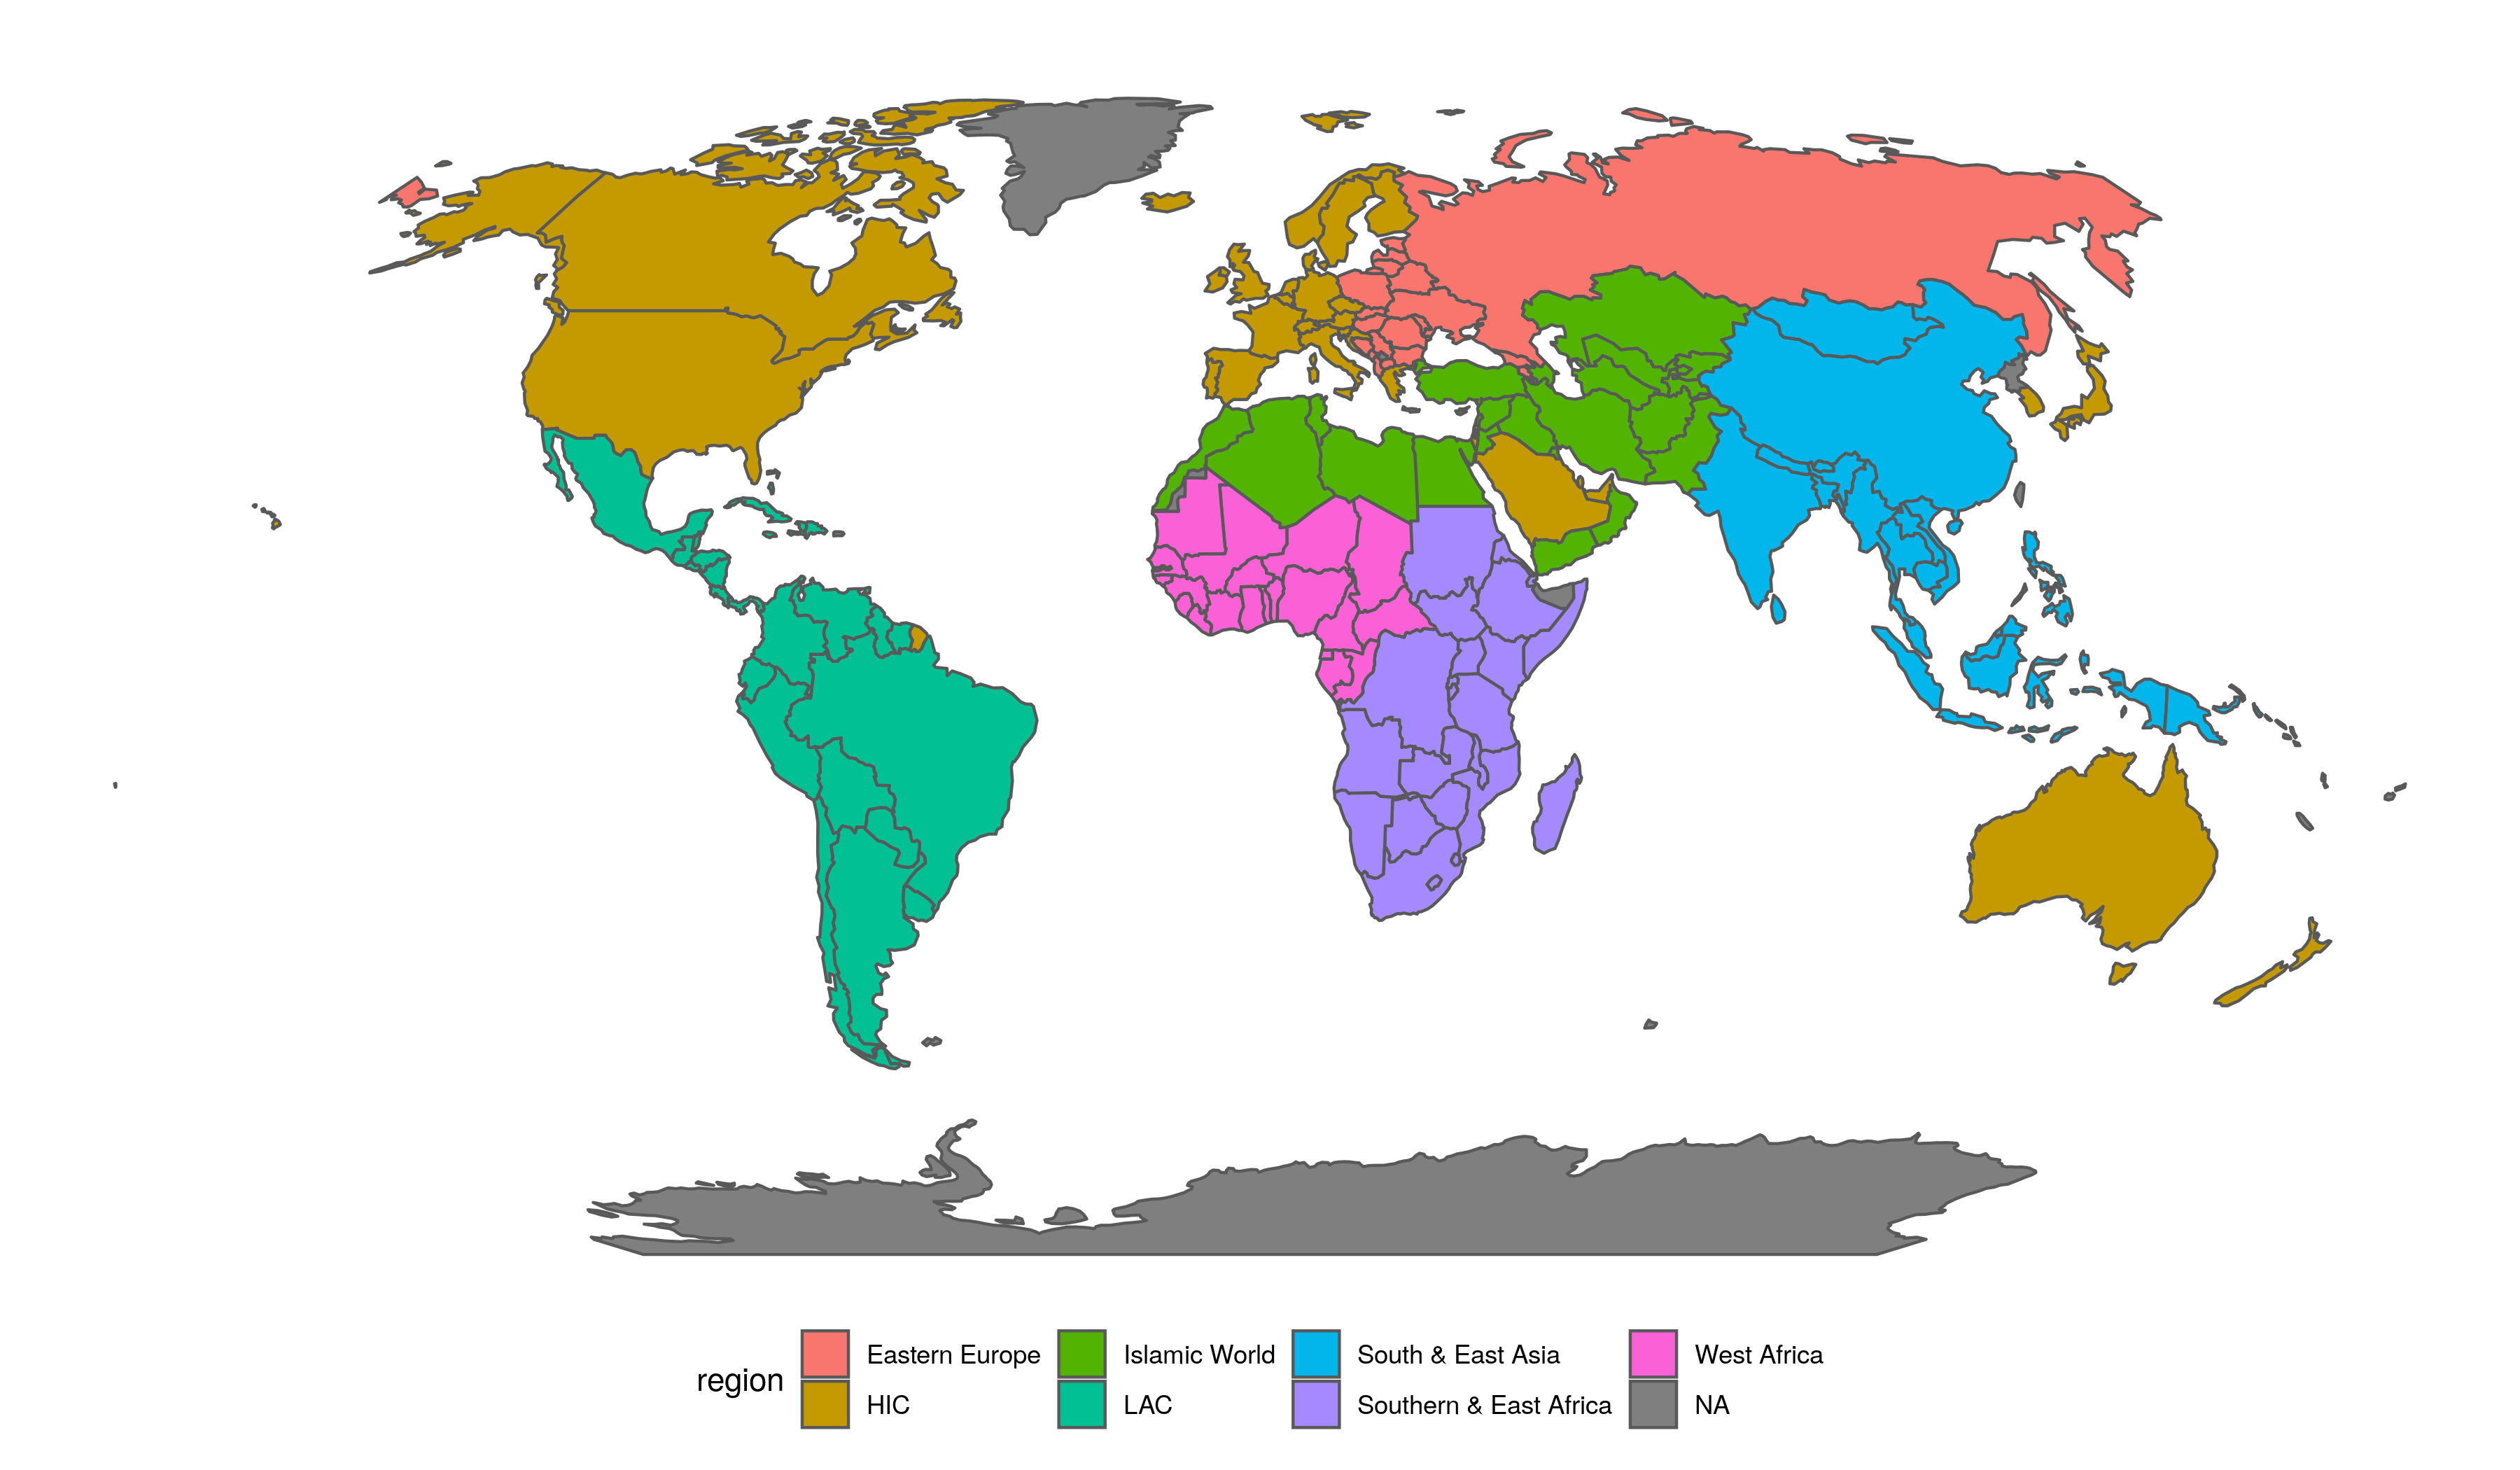
\includegraphics[width=\linewidth]{../figures/regions.png}
	\caption{Grouping used to estimate regional rates of food insecurity in urban and rural areas.}
	\label{fig:regions}
\end{figure}

\begin{figure}[h]
	\centering
	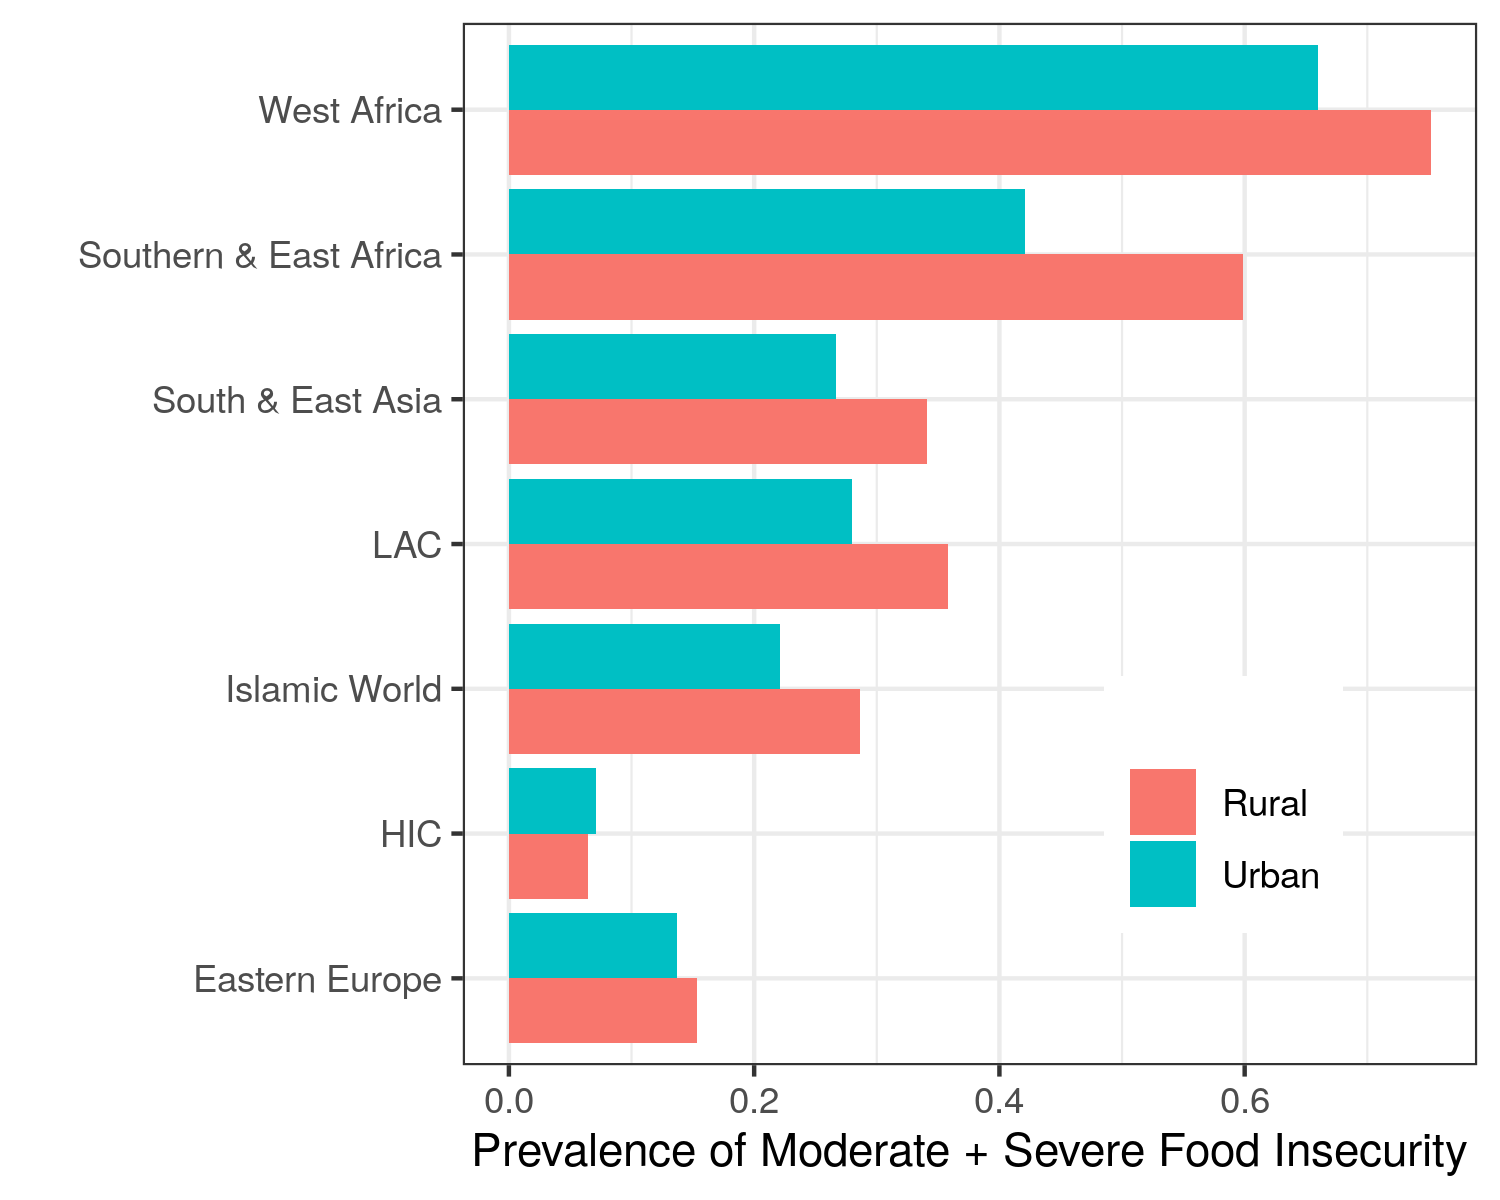
\includegraphics[width=0.75\linewidth]{../figures/Urban_Rural.png}
	\caption{Rates of food insecurity in urban and rural areas by world region.}
	\label{fig:regionrate}
\end{figure}

Examining rates of food insecurity by both urban and rural areas shows that, in nearly every world region, food insecurity is worse in rural areas, with the largest gap in Southern Africa.  High-income countries area the only exception, and food insecurity is actually worse in urban parts of these countries than in rural areas.

Given the overall rate of food insecurity in each country, the disparities in rates of urban and rural food insecurity in each world region, and the percentage of the population and urban and rural areas within each admin-1 area of each country, it is possible to derive a rate of food insecurity specific to each admin-1 area.

Formally, given the following two assumptions:

\begin{equation} 
\omega / \rho = ratio 
\label{eq1}
\end{equation}

\begin{equation} 
\omega * URB + \rho * RUR = t * TOT
\label{eq2}
\end{equation}
\newline

Where:

\begin{itemize}
	\item $\omega$: The percentage of households in urban areas in a country with food insecurity (UNKNOWN)
	
	\item $\rho$: The percentage of households in rural areas in a country with food insecurity (UNKNOWN)
	
	\item $t$: The overall percentage of households in a country with food insecurity (KNOWN)
	
	\item $RUR$: The total population in rural areas (KNOWN)
	
	\item $URB$: The total population in urban areas (KNOWN)
	
	\item $TOT$: The total population (KNOWN)
	
	\item $ratio$: The ratio of the rates of urban food insecurity to rural food insecurity.  This is known at a regional level, and it is estimated that the same ratio holds at the individual country level.
\end{itemize}

We can solve for the two unknown parameters, $\omega$ and $\rho$ to get country-level estimates of urban and rural rates of food insecurity and derive subnational prevalences.

Thus, we derive the following map of disaggregated rates of food insecurity in countries where we have direct FIES data (See Figure \ref{fig:disaggregated}).

\begin{figure}[h]
	\centering
	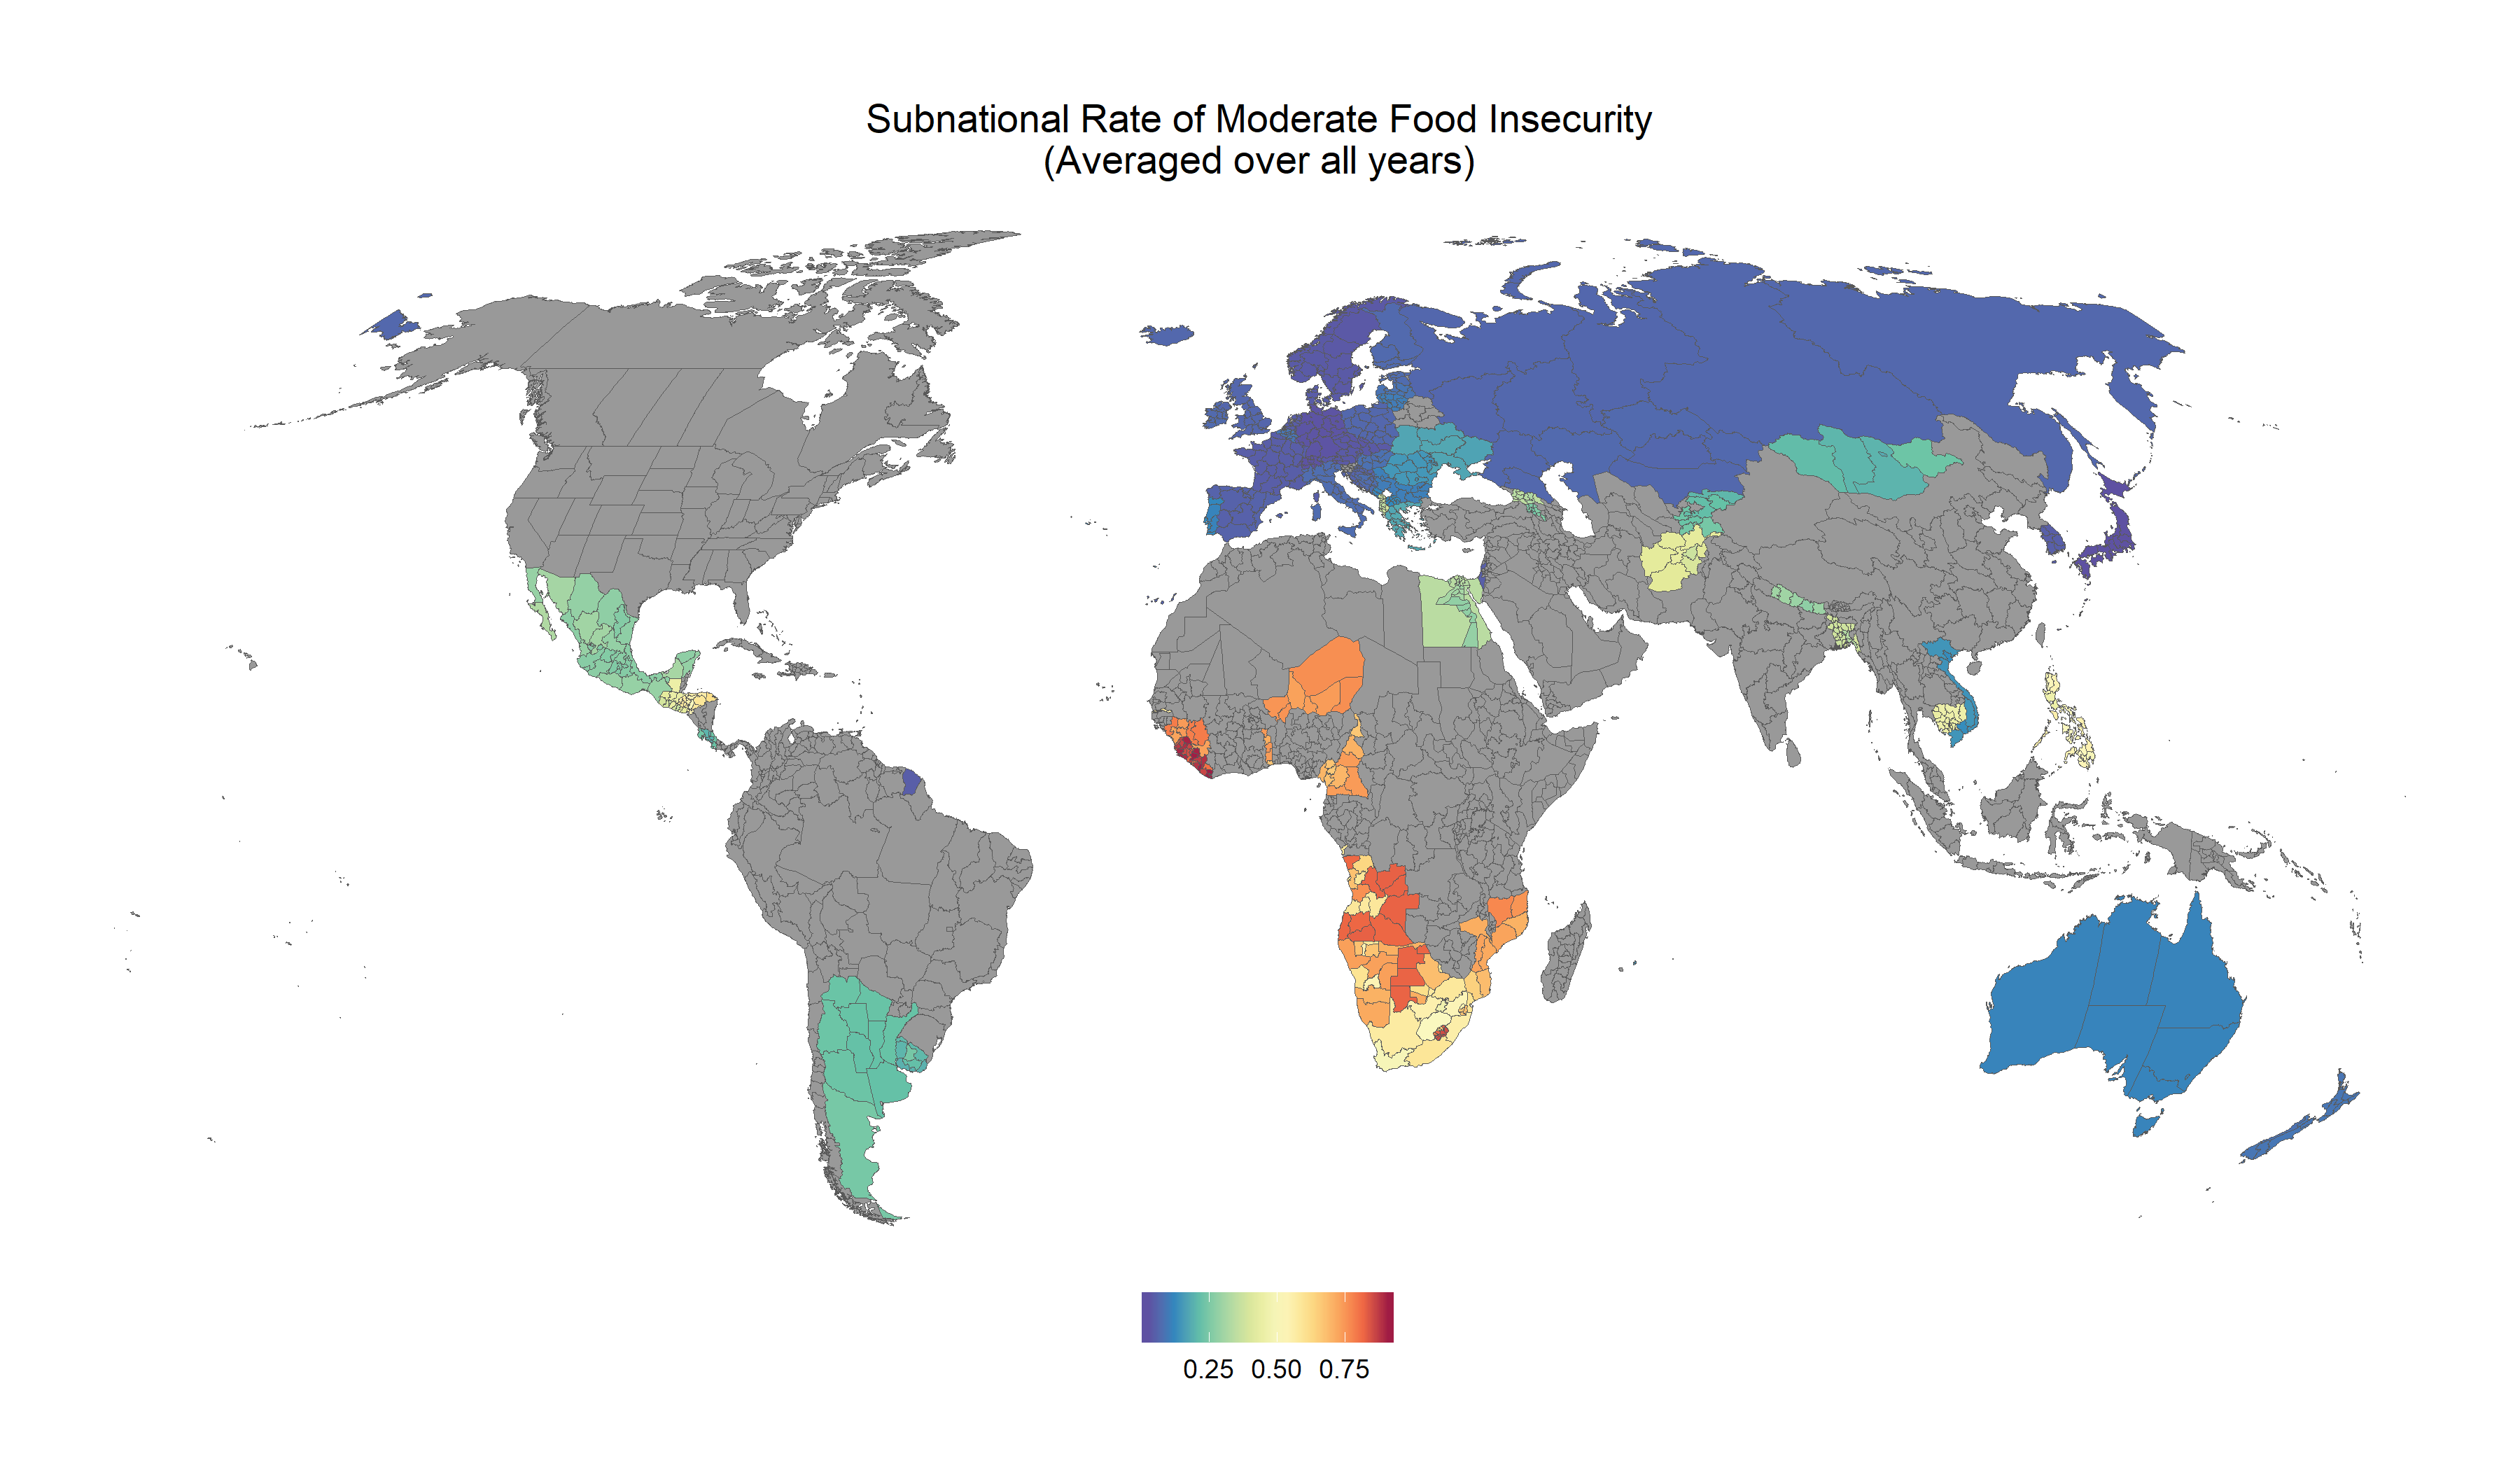
\includegraphics[width=\linewidth]{../figures/subnational-moderate.png}
	\caption{Rates of food insecurity in urban and rural areas by world region, averaged across all years for which survey data is available}
	\label{fig:disaggregated}
\end{figure}

\subsection{Modeling the FIES in the Present}
We then used these Admin-1 estimates, in combination with a large stack of covariates in the present, to model the prevalence of food insecurity globally for the year 2020, based on covariates for as close to the year 2020 as possible.  We used a LASSO regression approach, where the size of the regression coefficients are penalized, which is most appropriate for making predictions based on a large number of covariates \cite{Tibshirani2011}.

For our in-sample data, the LASSO performed well (see Figure \ref{fig:lasso_residuals}).  The coefficients for each variable are given in Figure \ref{fig:lasso_coefs}.  Note that some coefficients are penalized to 0, which effectively removes them from the model.  The map is the results is given in Figure \ref{fig:lasso_map}.

\begin{figure}[H]
	\centering
	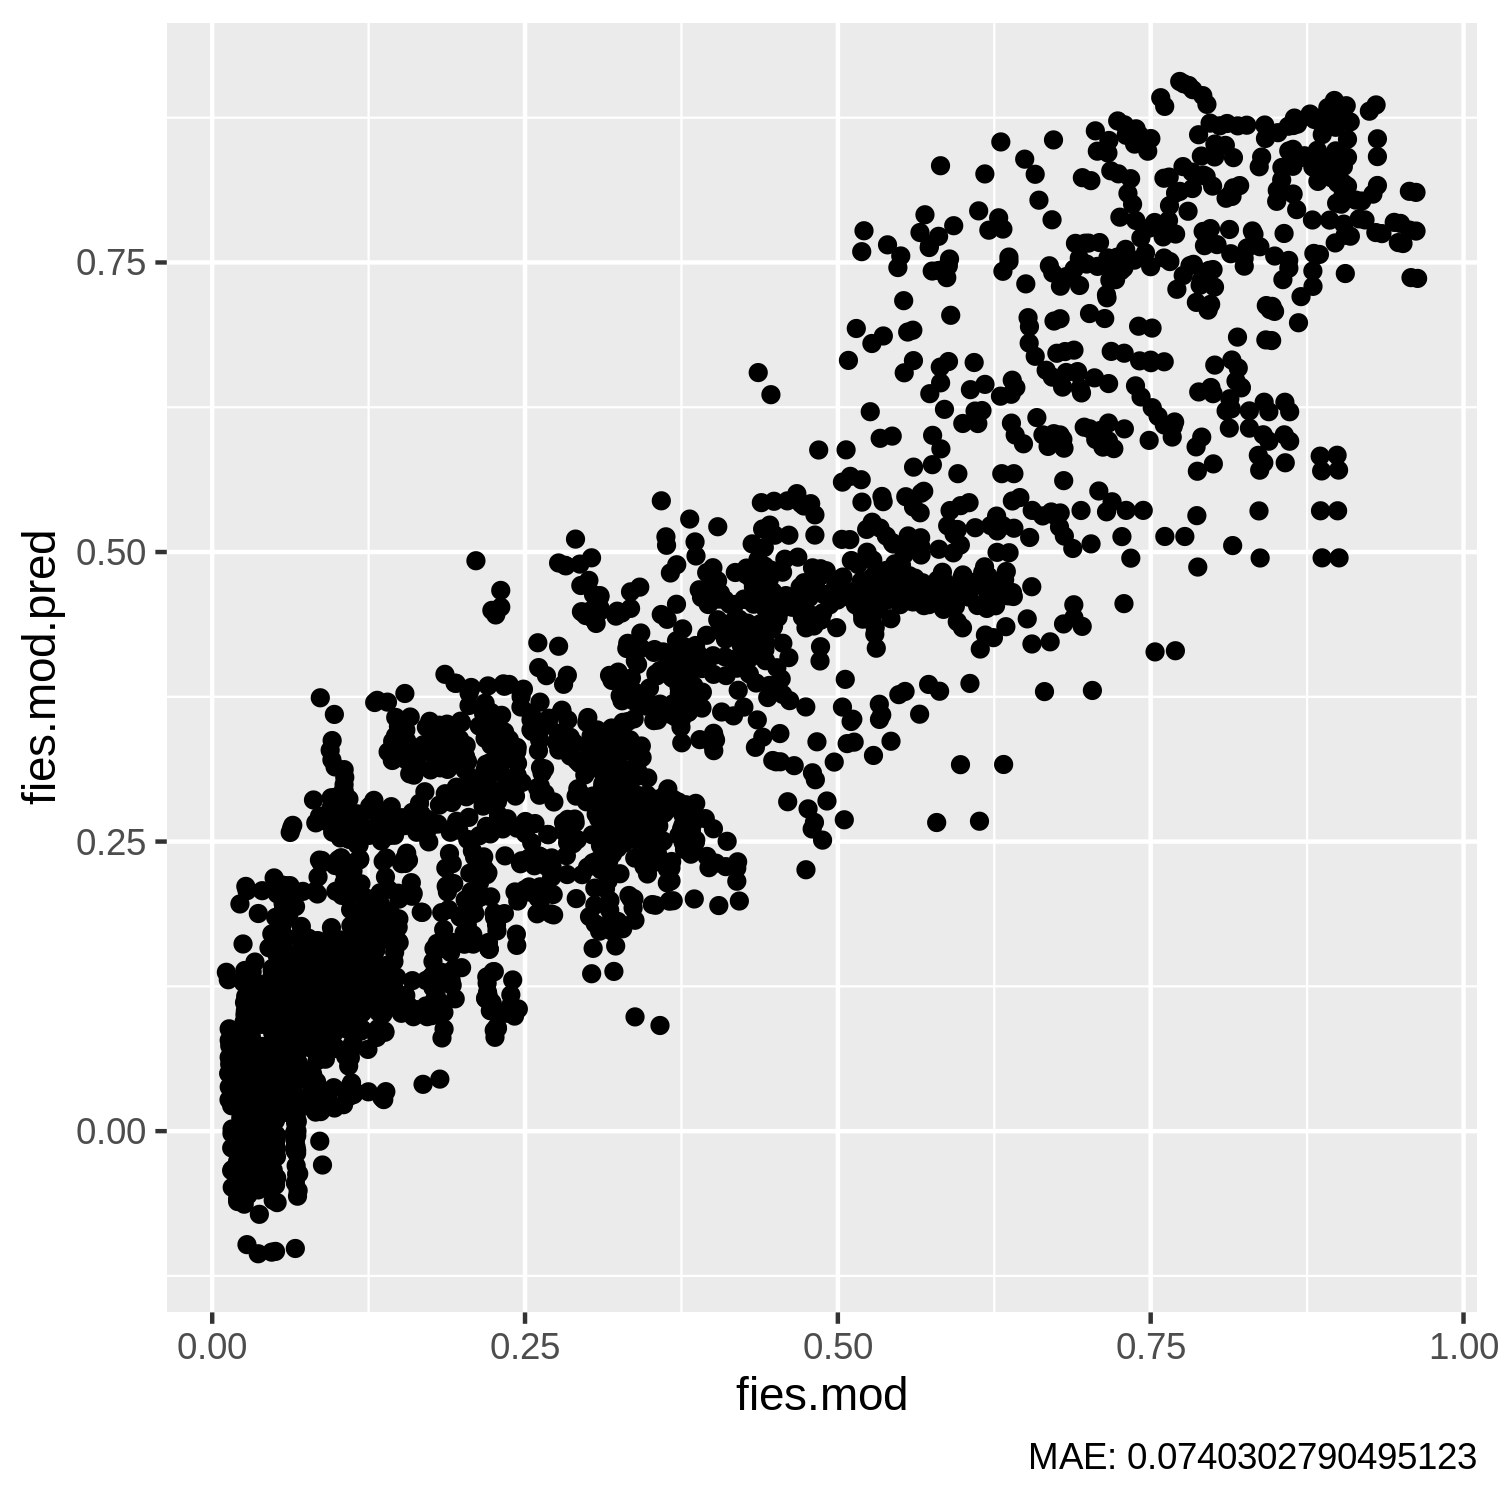
\includegraphics[width=0.6\linewidth]{../figures/Pred2020_Residuals.png}
	\caption{Correlation between observed disaggregated rates of food insecurity and modeled rates of food insecurity.}
	\label{fig:lasso_residuals}
\end{figure}
\begin{figure}[H]
	\centering
	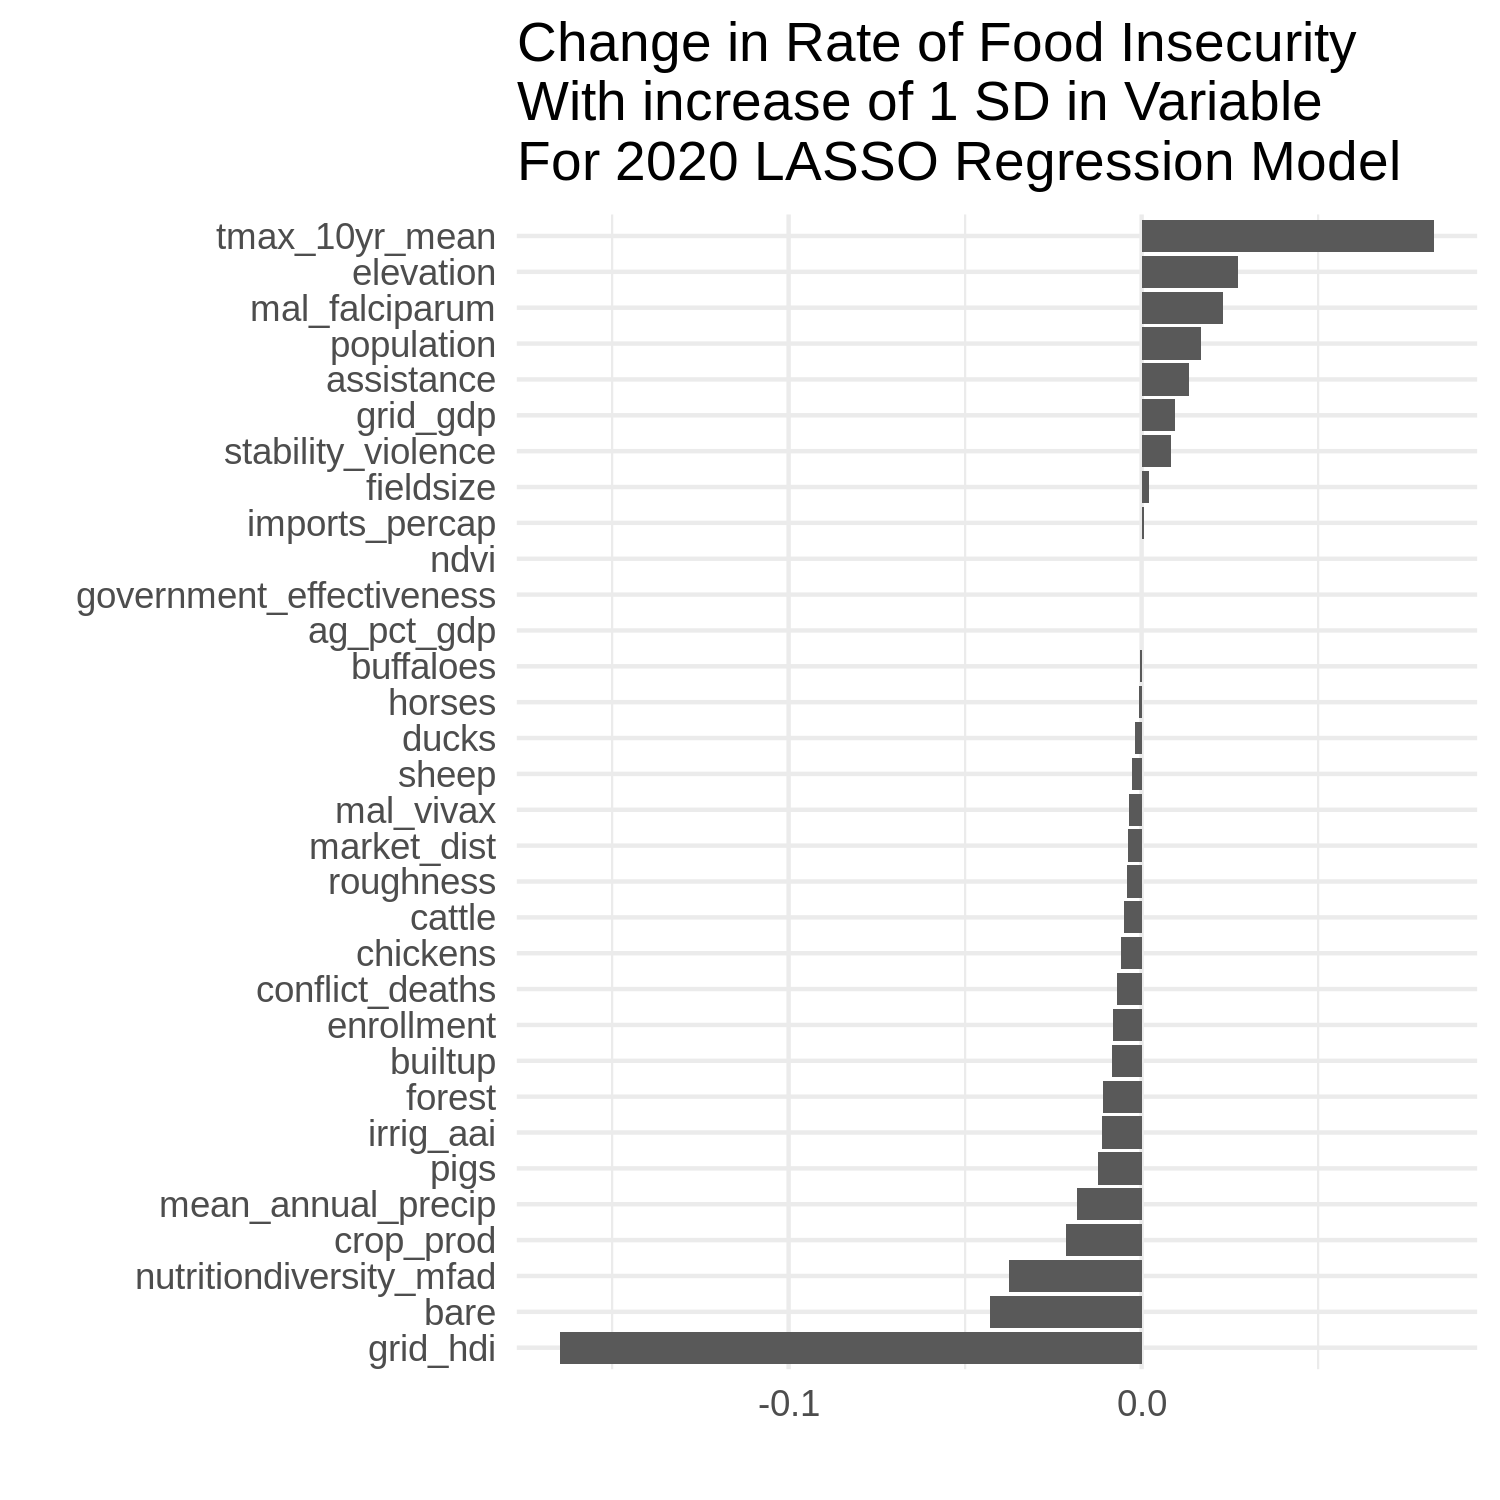
\includegraphics[width=0.6\linewidth]{../figures/Pred2020_Coefs.png}
	\caption{Change in rate of food insecurity with a 1 standard deviation increase in each variable.  NOTE: IN A FUTURE EDITION THE LABELS WILL BE BETTER.}
	\label{fig:lasso_coefs}
\end{figure}
\begin{figure}[H]
	\centering
	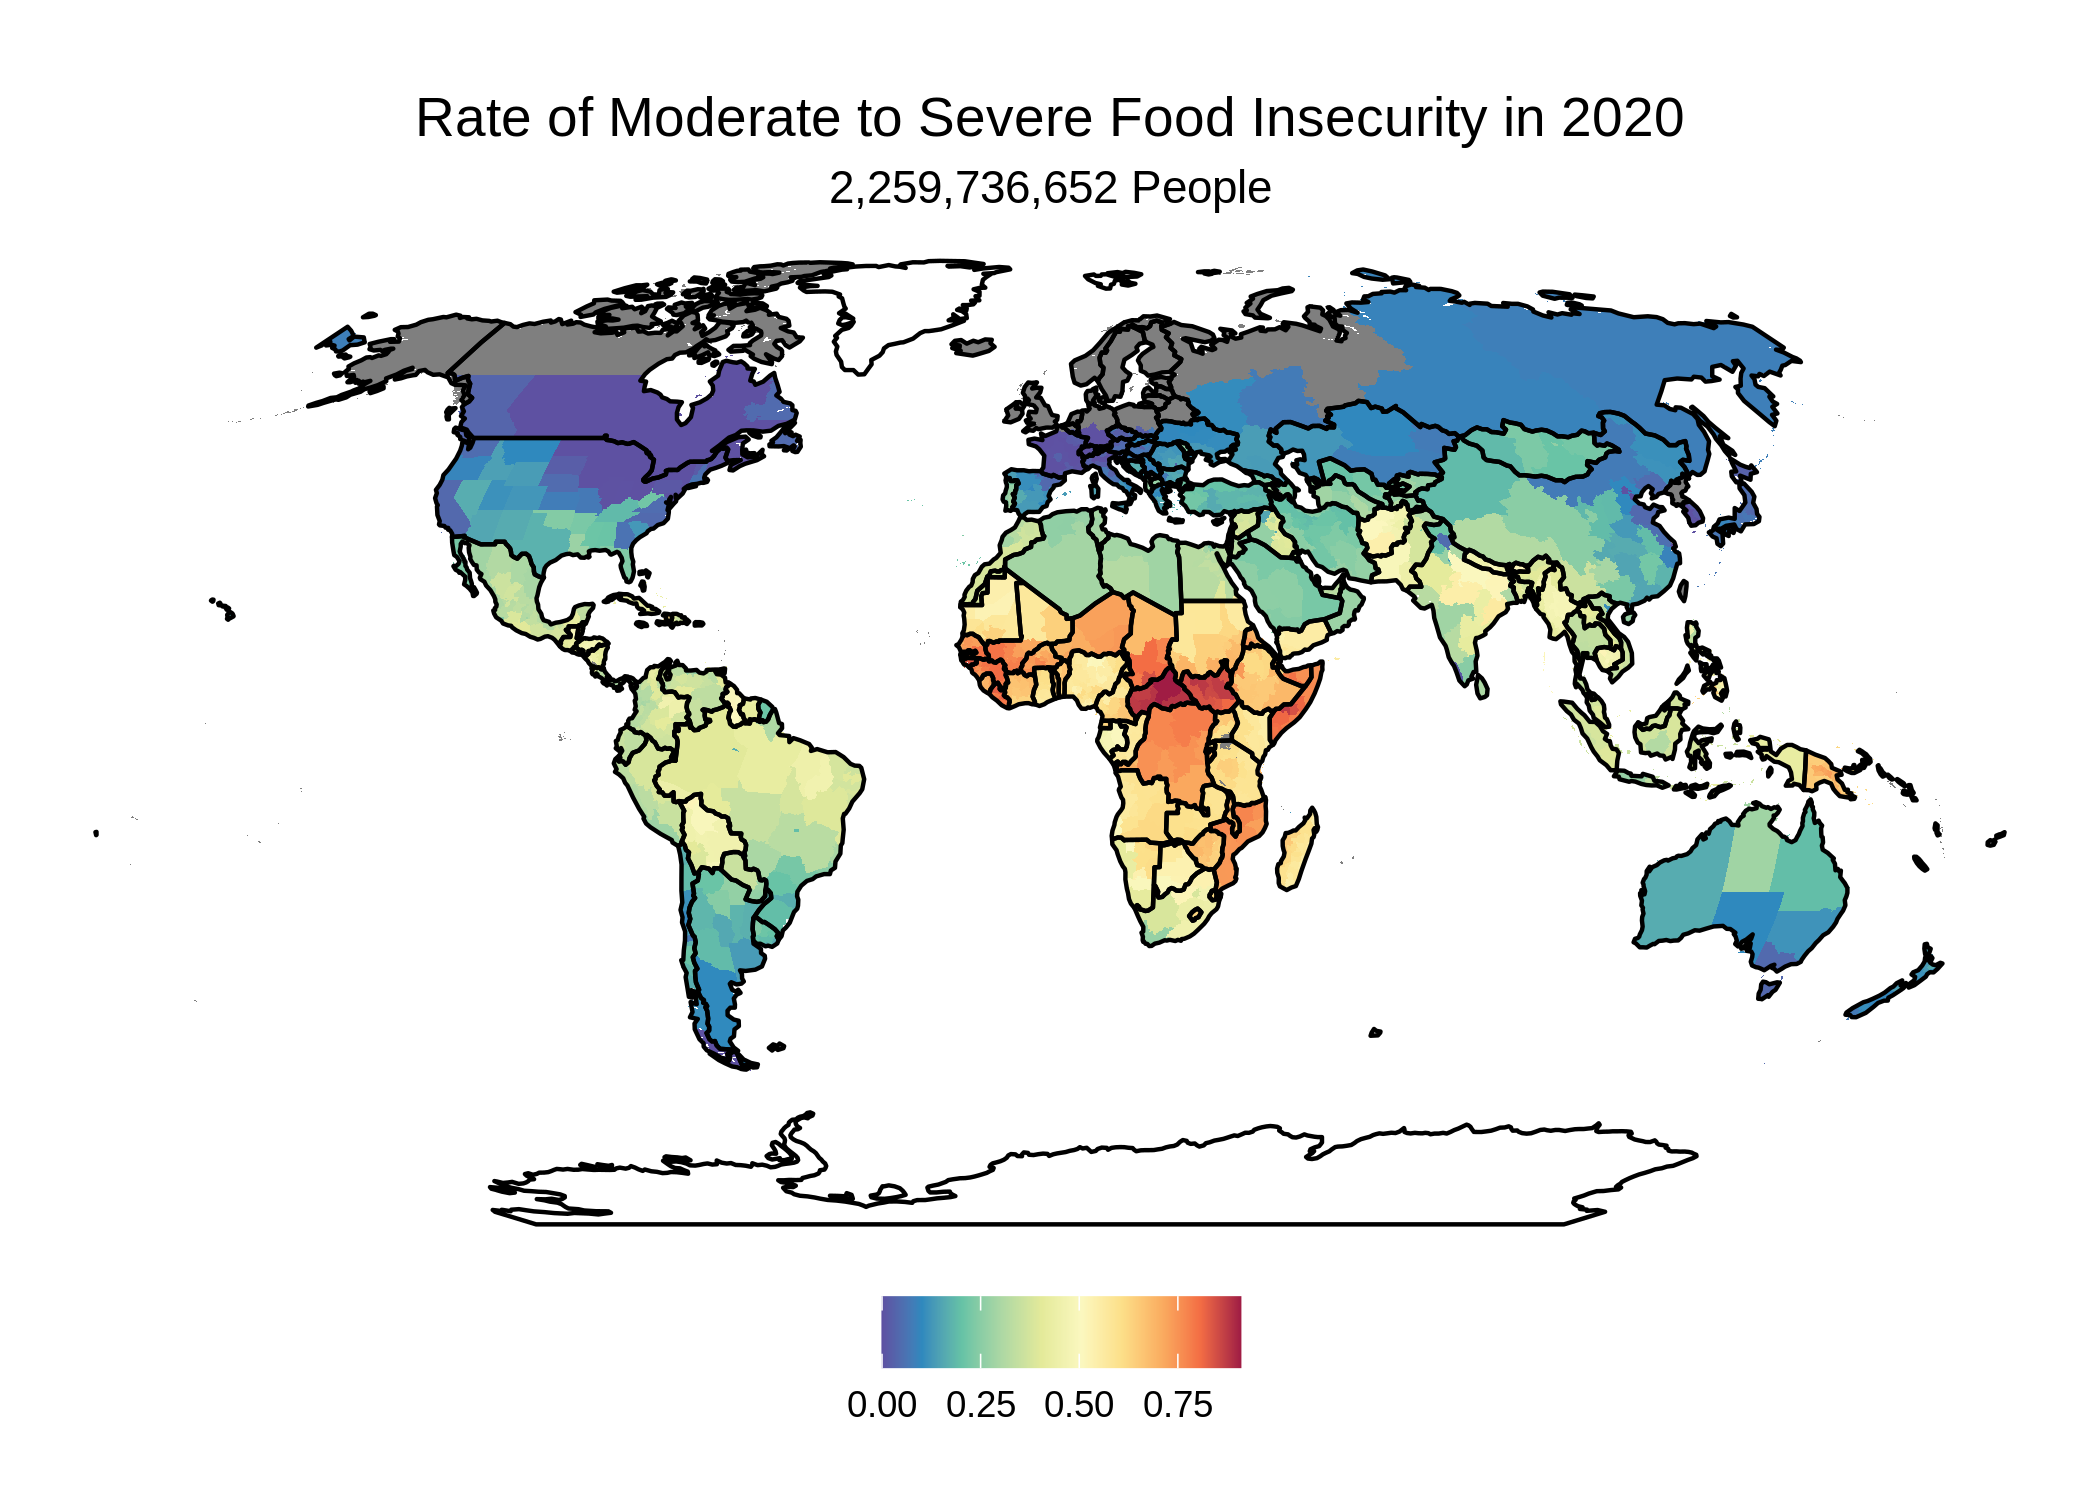
\includegraphics[width=\linewidth]{../figures/Pred2020_LASSO.png}
	\caption{Estimated rates of food insecurity in 2020. NOTE: SOME COVARIATES ARE MISSING AT HIGH LATITUDES, THIS WILL BE FIXED IN A FUTURE EDITION.}
	\label{fig:lasso_map}
\end{figure}


\subsection{Modeling the FIES in the Future}
In addition to modeling the FIES in the present, we also modeled the FIES for the years 2020, 2025, and 2030, based covariates that were already extrapolated to the year 2030 in peer-reviewed literature.  NOTE: MANY MORE COVARIATES ARE BEING ADDED.  Similar to the previous model, we below show the correlation between the observed and predicted values (Figure \ref{fig:ssp_residuals}), the estimated coefficients (Figure \ref{fig:ssp_coefs}), and the mapped results (Figure \ref{fig:ssp_map}).


\begin{figure}[H]
	\centering
	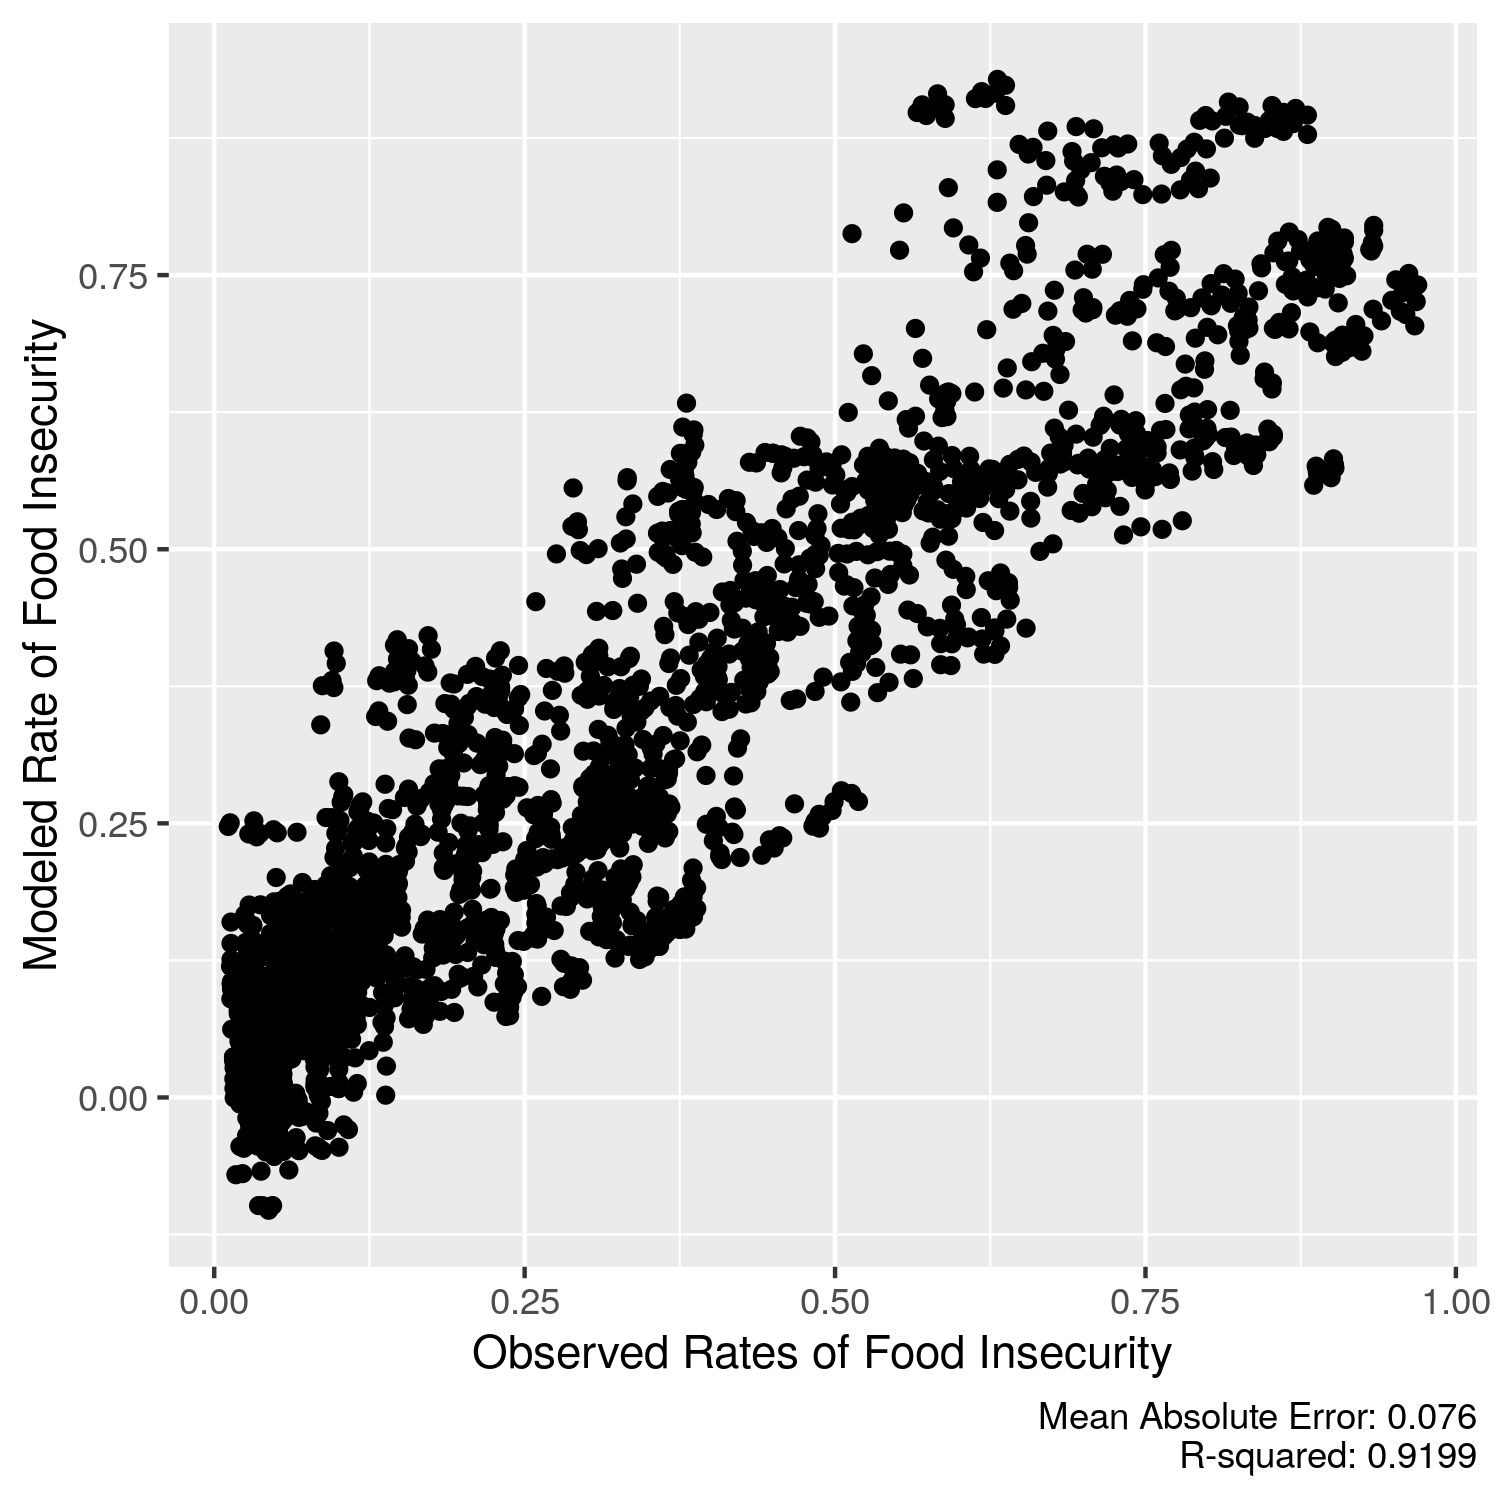
\includegraphics[width=0.6\linewidth]{../figures/SSP2_Residuals.png}
	\caption{Correlation between observed disaggregated rates of food insecurity and modeled rates of food insecurity.}
	\label{fig:ssp_residuals}
\end{figure}
\begin{figure}[H]
	\centering
	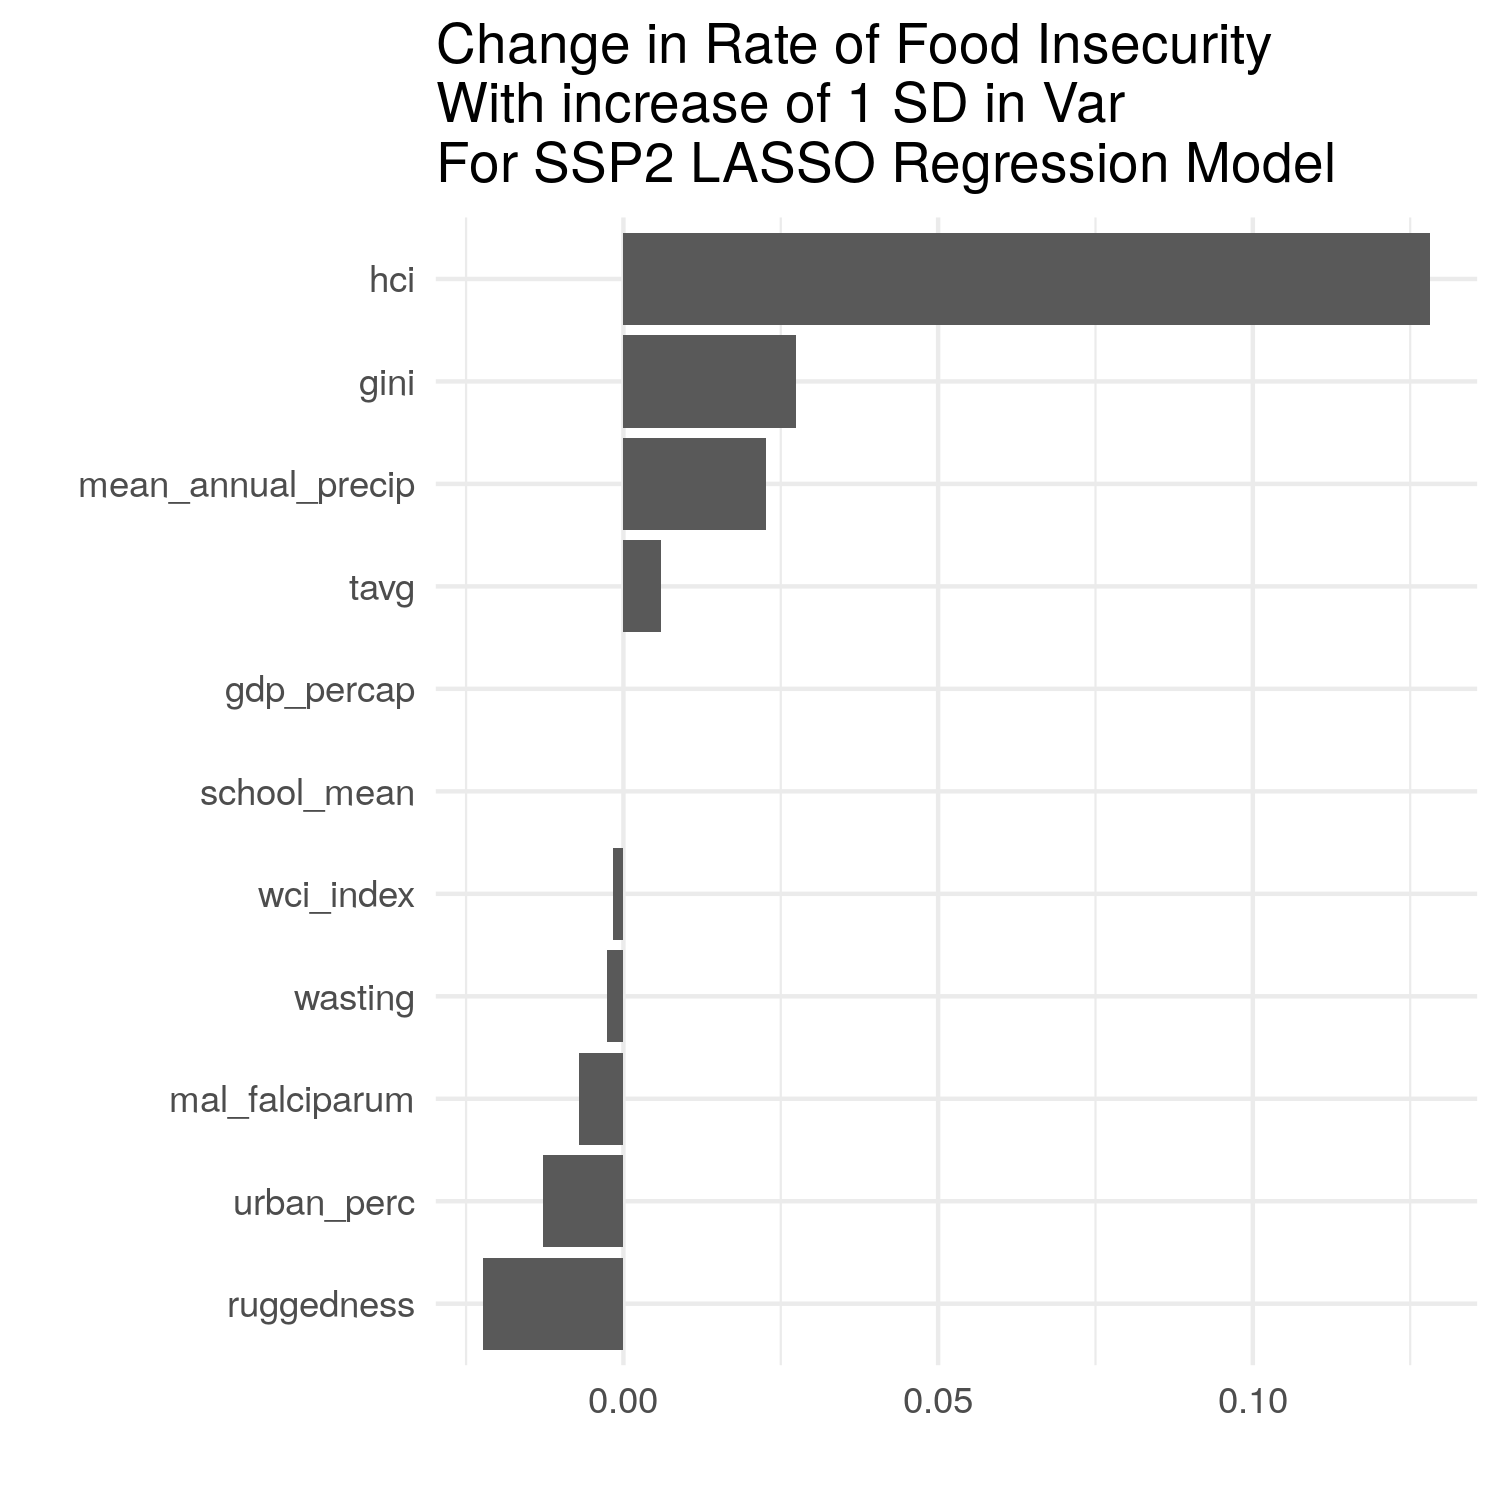
\includegraphics[width=0.6\linewidth]{../figures/SSP2_Coefs.png}
	\caption{Change in rate of food insecurity with a 1 standard deviation increase in each variable.  NOTE: IN A FUTURE EDITION THE LABELS WILL BE BETTER AND MORE COVARIATES WILL BE INCLUDED.}
	\label{fig:ssp_coefs}
\end{figure}
\begin{figure}[H]
	\centering
	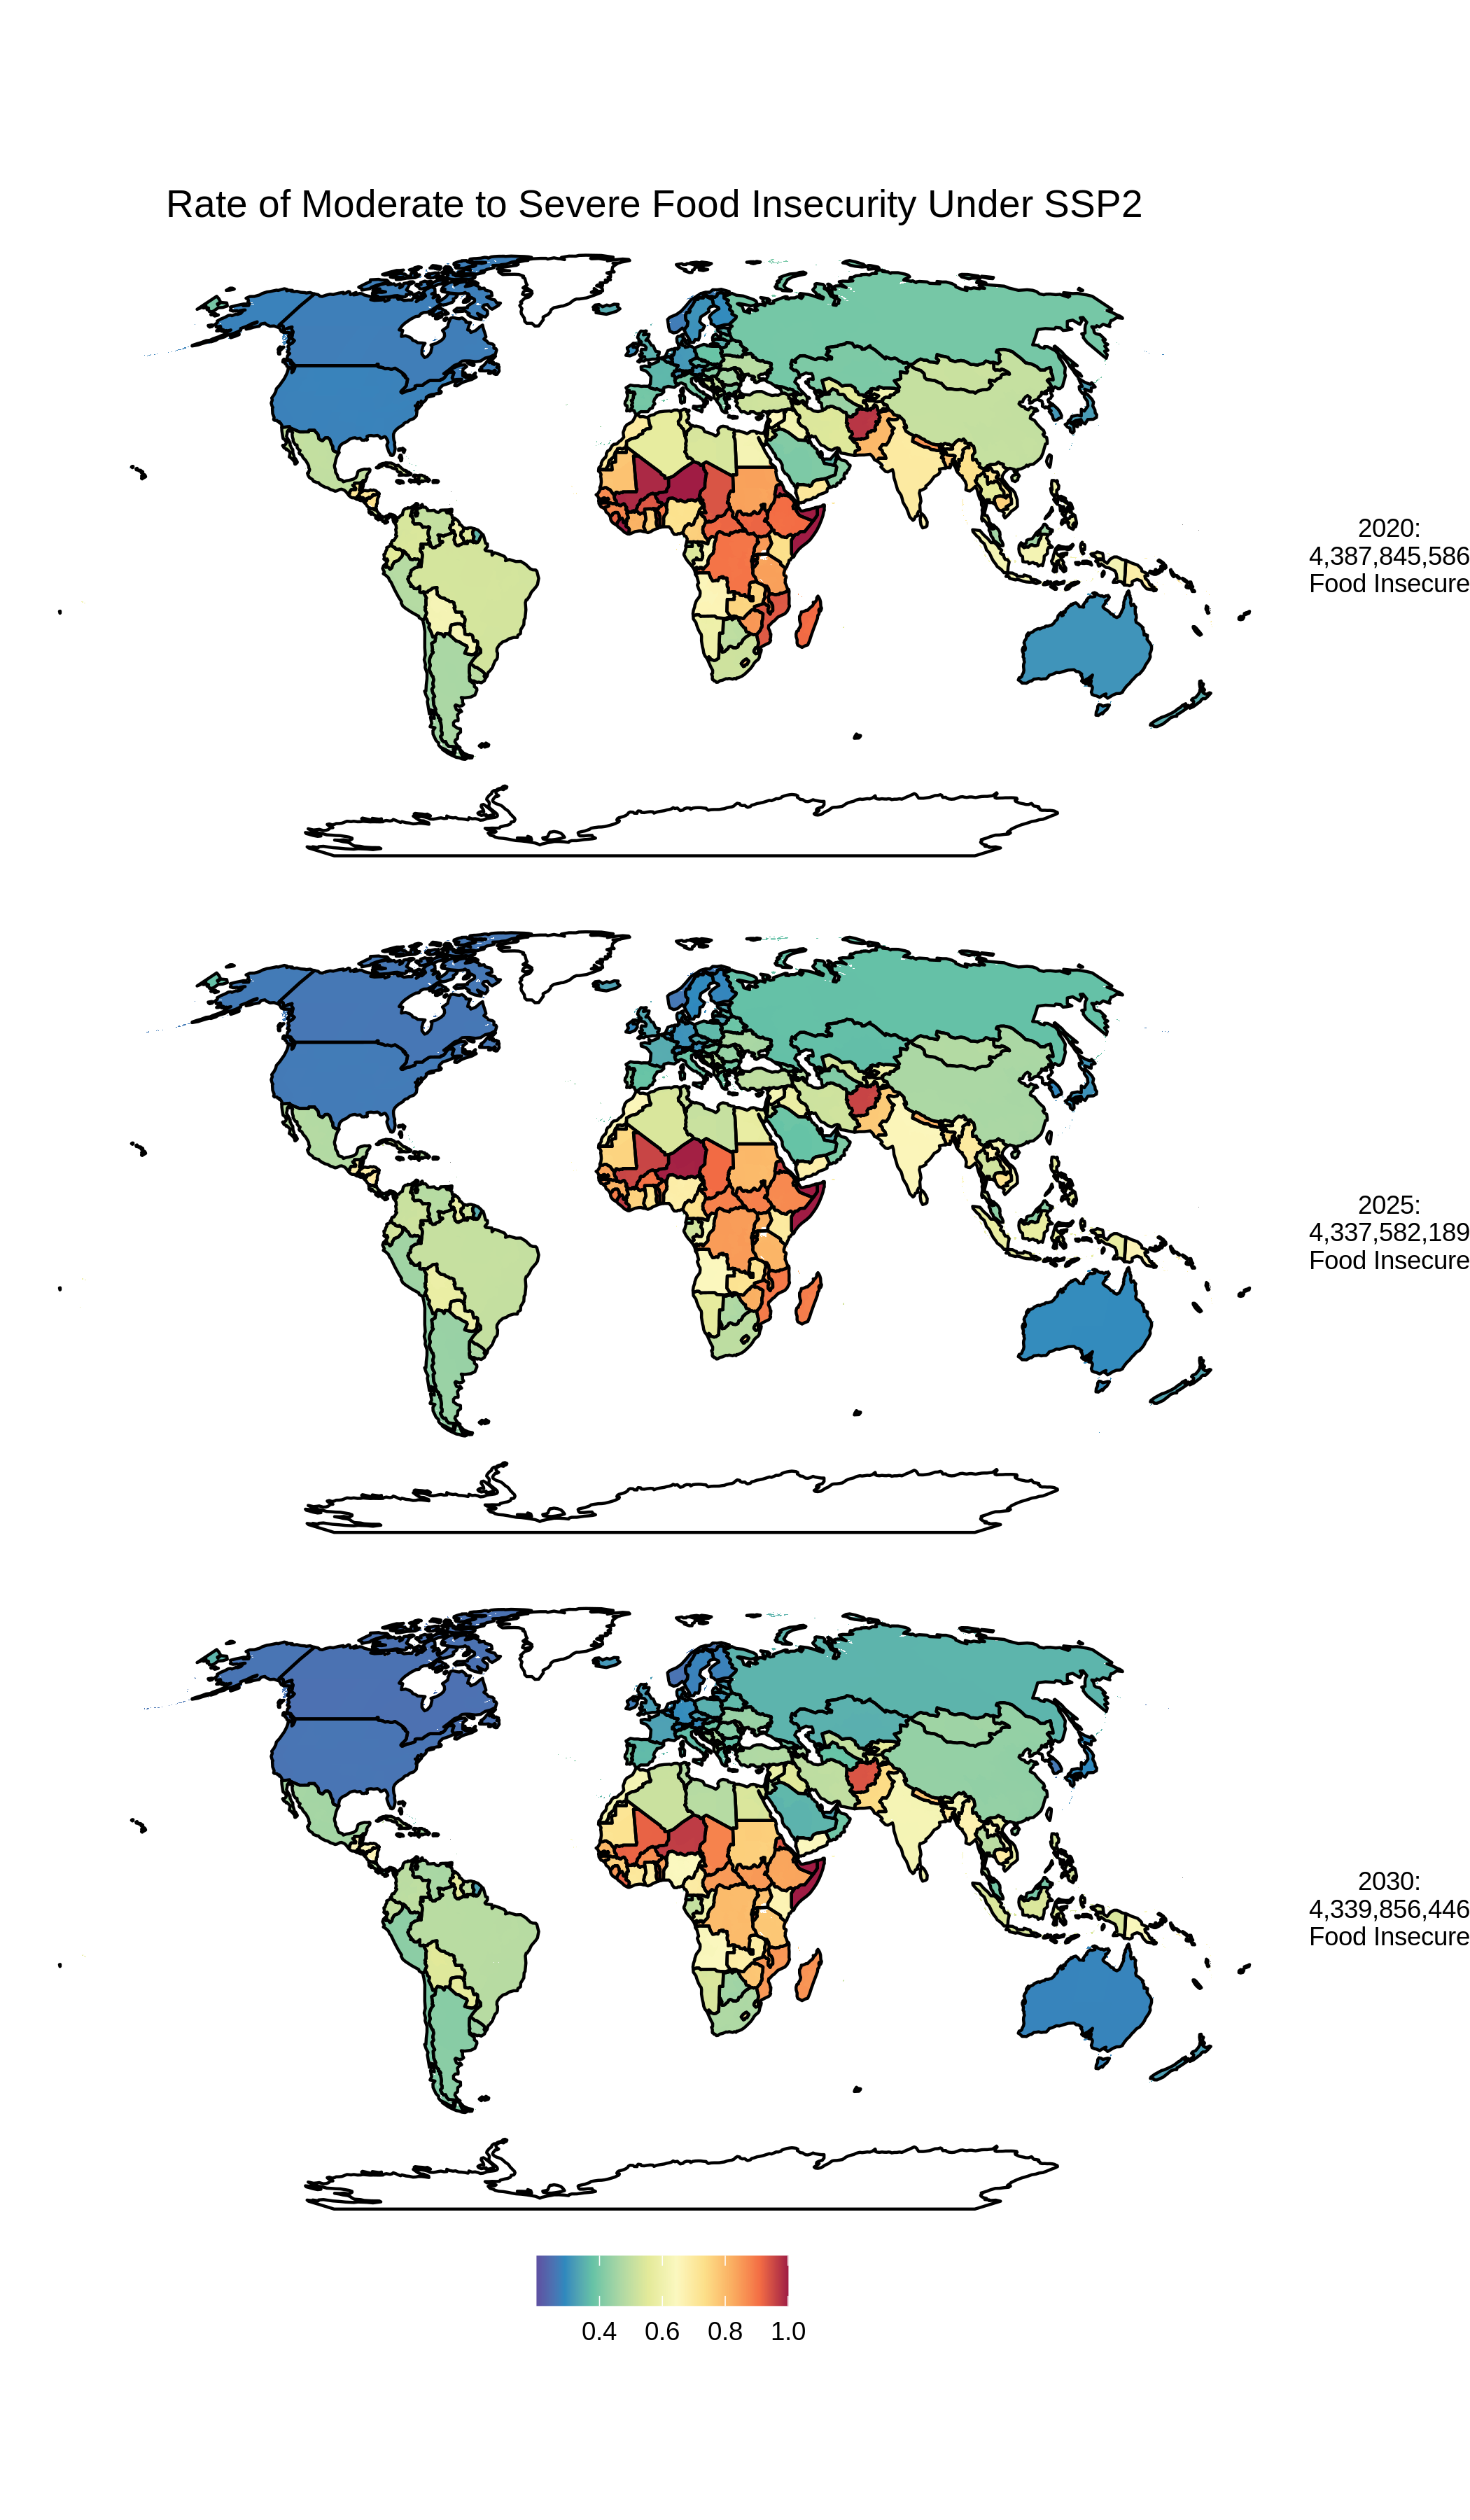
\includegraphics[width=\linewidth]{../figures/SSP2_LASSO.png}
	\caption{Estimated rates of food insecurity in 2020, 2025, and 2030.}
	\label{fig:ssp_map}
\end{figure}

\section{Discussion}
There is still a wide gap between the predictions of the 2020 model based on the large stack of covariates and the 2020 model based on just the SSP covariates.

\section{Conclusion}

\clearpage
\bibliographystyle{apalike}

%Determine local environment
\bibliography{references}


\section*{Supplemental Info}


\end{document}